\chapter{Musikteori}
I dette kapitel introduceres grundlæggende musikteori, der anvendes i projektet.
\\ \\
I nodesystemet er en node en symbolsk repræsentation af en bestemt tone, som er tilknyttet en specifik frekvens (angivet i hertz, Hz). Hver node indeholder således information om tonens højde og desuden også om dens varighed. Et nodeark er således en symbolsk repræsentation af et diagram over tid og frekvens, hvilket også kaldes et spektrogram.
\\ \\
Til at notere noder benytter man et nodesystem, der består af fem vandrette linjer, hvor noderne er placeret. Grundlæggende findes der 12 forskellige toner Noderne i nodesystemet består først og fremmest af stamtoner, som navngives med bogstaverne A-G afhængigt af deres vertikale placering. Efter G starter navngivningen forfra med det næste A, der ligger en oktav over det forrige. Mellem flere af stamtonerne ligger andre toner, som sammen med stamtonerne udgør de 12 grundtoner, som typisk anvendes i musik. Afstanden mellem alle grundtonerne er en halv tone.

\begin{figure}[H]
    \centering
    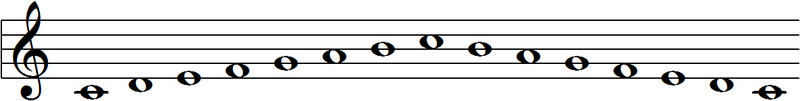
\includegraphics[width = 0.6\textwidth]{figures/C_dur.PNG}
    \caption{C-dur.}
    \label{Cdur}
\end{figure}
